\documentclass{article}

% if you need to pass options to natbib, use, e.g.:
% \PassOptionsToPackage{numbers, compress}{natbib}
\PassOptionsToPackage{square,numbers}{natbib}
\bibliographystyle{abbrvnat}
% before loading nips_2016
%
% to avoid loading the natbib package, add option nonatbib:
% \usepackage[nonatbib]{nips_2016}

% \usepackage{nips_2016}

% to compile a camera-ready version, add the [final] option, e.g.:
\usepackage[final]{nips_2016}

\usepackage{enumitem}
\usepackage[utf8]{inputenc} % allow utf-8 input
\usepackage[T1]{fontenc}    % use 8-bit T1 fonts
\usepackage[hidelinks]{hyperref}       % hyperlinks
\usepackage{url}            % simple URL typesetting
\usepackage{booktabs}       % professional-quality tables
\usepackage{amsfonts}       % blackboard math symbols
\usepackage{nicefrac}       % compact symbols for 1/2, etc.
\usepackage{microtype}      % microtypography
\usepackage{mathtools}
\usepackage{placeins}
\usepackage{float}
\usepackage{graphicx}
\usepackage{color}
\usepackage{amsthm}
\usepackage{mmstyles}
\DeclareGraphicsExtensions{.pdf,.png,.jpg}

\newcommand{\misscite}{\textcolor{red}{[CITE]}}
\newcommand{\missref}{\textcolor{red}{REF}}
\newcommand{\todo}{\textcolor{red}{TODO}}
\newcommand{\real}{{\mathbb{R}}}
\newcommand{\zz}{{\mathbb{Z}}}
\newcommand{\bt}{{\mathbf{t}}}
\newcommand{\bx}{{\mathbf{x}}}
\newcommand{\by}{{\mathbf{y}}}
\newcommand{\bu}{{\mathbf{u}}}
\newcommand{\bg}{{\mathbf{g}}}
\newcommand{\bh}{{\mathbf{h}}}
\newcommand{\bR}{{\mathbf{R}}}
\newcommand{\E}{{\mathbb{E}}}
\newcommand{\row}{{\text{row}}}
\newcommand{\col}{{\text{col}}}
\newcommand{\nullsp}{{\text{null}}}
\newcommand{\Mbar}{{\overline{\M}}}
\newcommand{\prob}{{\text{Pr}}}

\title{SEEM 5380 Lecture Notes}

% The \author macro works with any number of authors. There are two
% commands used to separate the names and addresses of multiple
% authors: \And and \AND.
%
% Using \And between authors leaves it to LaTeX to determine where to
% break the lines. Using \AND forces a line break at that point. So,
% if LaTeX puts 3 of 4 authors names on the first line, and the last
% on the second line, try using \AND instead of \And before the third
% author name.

\author{
	Anthony Man-Cho So \\
}

\begin{document}
	% \nipsfinalcopy is no longer used

\maketitle

\section{Note 1}

\subsection{Prelude}

\subsubsection{Recall}

Regularized loss minimization
% Q
\footnote{examples?}
\begin{equation}
\hat\theta \in \argmin_{\theta\in\real^d} \{\cL(\theta;\{z_i\}_{i=1}^n) + \lambda R(\theta)\}
\end{equation}
for estimating a certain unknown vector $\theta^*\in\real^d$.
Here $z_1,\dots,z_n$ are iid \wrt $\Pbb_{\theta^*}$.
% Q
\footnote{what does notation $\Pbb_{\theta^*}$ mean?}
Denote
\begin{equation}
F := \cL(\theta;\{z_i\}_{i=1}^n) + \lambda R(\theta).
\end{equation}

\subsubsection{This Lecture}

Derive bounds on the statistical error
% Q
\footnote{what is a \emph{statistical error}?}
$\hat\Delta = \hat\theta - \theta^*$.

\subsubsection{Motivation}

\begin{itemize}
    \item From optimization, expect
        $|F(\hat\theta) - F(\theta^*)|$
        to be small.
        % Q
        \footnote{why it should small? why from optimization?}
    \item Show that $\hat\Delta$ belongs to a region
        that $F$ is not too flat.
        % Q
        \footnote{we want $\hat\Delta$ be small,
        so we expect $F$ not flat near origin?}
        This involves accounting fo the effect of $R$.
    \item $R$ is intended to promote certain desirable structure (\eg sparsity).
        We need to know how $R$ penalizes deviation,
        which leads to the \emph{decomposability} concept.
\end{itemize}

\subsubsection{Decomposability of $R$}

\begin{itemize}
    \item $\cM$: model subspace,
        which captures the constraints specified by the model
        (\eg vectors within certain support for sparsity).
    \item Let $\cM \subset \cMbar \subset \real^d$ be a pair of subspaces.
        The \emph{perturbation subspace} is
        \begin{equation}
            \cMbar^\perp = \{v\in\real^d: u^Tv=0, \forall u\in\cMbar\}.
        \end{equation}
\end{itemize}

\begin{define}
    $R$ is decomposable \wrt $(\cM, \cMbar^\perp)$ if
    \begin{equation}
        R(\theta+\gamma) = R(\theta) + R(\gamma) \quad
        \forall \theta \in \cM, \gamma \in \cMbar^\perp.
    \end{equation}
\end{define}

\begin{obs} \leavevmode
\begin{itemize}
    \item $R$ is a norm and hence
        $R(\theta+\gamma)\le R(\theta) + R(\gamma)$.
        This means we want the perturbation term $\gamma$ be
        maximally penalized (up to the equal sign).
        % N
        \footnote{seems to me this maximally penalization is just an excuse for
        the simplified assumption.}
    \item The notion of decomposability is useful when $\cM$ is small,
        in the sense that $\Pi_\cM(\theta^*)\approx\theta^*$.
        % N
        \footnote{i think the sense of small is strange since when
        $\cM$ is large enough, that projection would be exact.
        Should we phrase it as
        \emph{it is useful when $\cM$ is small and
        at the same time not being too far from $\theta^*$}?}
\end{itemize}
\end{obs}

\begin{ex}[Sparse vectors and $l_1$-regularization] \leavevmode
\begin{itemize}
    \item model: $S$-sparse vectors in $\real^d$, $R(\theta)=\|\theta\|_1$.
    \item for any $S\subset\{1,\dots,d\}$ of cardinality $s$,
        define $\cM(S):=\{\theta\in\real^d:\theta_j=0\ \forall j \notin S \}$.
        If $\theta^*$ is supported on $S$,
        then $\Pi_{\cM(S)}(\theta^*)=\theta^*$.
    \item take $\cMbar(S):=\cM(S)$,
        so $\cMbar(S)^\perp = \cM(S)^\perp$.
        % N
        \footnote{notation $\cMbar(S)^\perp$ corrected from $\cMbar^\perp(S)$ (undefined).}
    \item decomposability is obvious.
\end{itemize}
\end{ex}

\begin{ex}[Group-structured norms] \leavevmode
\begin{itemize}
    \item motivation: groups of coefficients likely to be
        zero or non-zero simultaneously.
    \item model: partition $\{1,\dots,d\}$ into $N$ disjoint groups
        $\{G_1,\dots,G_N\}$, number of selected groups should be small,
        say $s$; \ie $S\subset \{1,\dots,N\}$
        are the group indices that correspond to non-zero groups and $s=|S|$.
        The norm is
        \begin{equation}
            R(\theta) = \|\theta\|_{g,p} = \sum_{i=1}^N\|\theta_{G_i}\|_p,\quad p \in[1,\infty].
        \end{equation}
    \item subspace: for any $S\subset\{1,\dots,N\}$, set
        \begin{gather}
            \cM(S) := \{\theta\in\real^d:\theta_{G_i}=0, \forall i\notin S\}, \\
            \cMbar(S) := \cM(S).
        \end{gather}
    \item decomposability can be verified.
\end{itemize}
\end{ex}

\subsubsection{Key Consequences of Decomposability}

\begin{pro} Suppose $\cL$ is convex, differentiable,
    $\lambda\ge 2R^*(\nabla\cL(\theta^*;\{z_i\}_{i=1}^n))$
\end{pro}


\clearpage
\section{Note 2}
Reading~\cite{raskutti2010restricted}.

\subsection{Prelude}

\subsubsection{Recall}

We are interested in establishing the following \emph{restricted eigenvalue} (RE) condition:

\begin{equation}
    \frac{\|X\Delta\|_2^2}{2n}\ge \kappa\|\Delta\|_2^2\quad\forall\Delta\in\cC=
        \{\Delta\in\real^d:\|\Delta_{S^c}\|_1\le3\|\Delta_S\|_1\},
\end{equation}
where $\kappa>0$, $X\in\real^{n\times d}$.

In general,
one would not expect it to hold for arbitrary $X$;
\eg fix $\Delta\in\cC$ and construct $X$
\st $\Delta\in\nullsp(X)$.
Thus some assumptions on $X$ are needed.

Let us assume that the rows of $X$ are iid $\cN(0,I)$.
Our goal is to prove

\begin{thm}
    With prob. $\ge 1-c_1\exp(-c_2 n)$,
    for some $c_1,c_2>0$.
    \begin{equation}
        \frac{\|X\Delta\|_2}{\sqrt{n}}\ge
            \frac{1}{4}\|\Delta\|_2-9\sqrt{\frac{\log d}{n}}\|\Delta\|_1
            \quad \forall \Delta\in\real^d.
    \end{equation}
\end{thm}

Note that the theorem trivially holds for $\Delta=0$.
Thus without loss of generality,
we may assume $\|\Delta\|_2=1$.
The proof of the theorem consists of three main steps:

\paragraph{Step 1.}
For a given $r>0$, define
\begin{equation}
    V(r)=\{\Delta\in\real^d:\|\Delta\|_2=1,\|\Delta\|_1\le r\}.
\end{equation}
\begin{pro}\label{pro:b1}
    \begin{equation}
        \Ebb\bigg[\inf_{\Delta\in V(r)}\frac{\|X\Delta\|_2}{\sqrt{n}}\bigg]\ge
            3\bigg[\frac{1}{4}-\sqrt{\frac{\log d}{n}}r\bigg],
    \end{equation}
    whenever $V(r)\neq \emptyset$.
\end{pro}
\begin{proof}
The quantity of interest here is
\begin{equation}
    \widetilde Q(r,X) = \inf_{\Delta\in V(r)}\|X\Delta\|_2
        = \adjustlimits\inf_{\Delta\in V(r)}\sup_{u\in S^{n-1}}u^TX\Delta.
\end{equation}
Note that for each $(u,\Delta)\in S^{n-1}\times V(r)$,
\begin{equation}
Y_{u,\Delta}=u^TX\Delta
\end{equation}
is a zero mean Gaussian RV.
To get a lower bound on $\Ebb[\widetilde Q(r,X)]$,
or equivalently,
an upper bound on
\begin{equation}
    \Ebb[-\widetilde Q(r,X)] =
        \Ebb\bigg[\adjustlimits\sup_{\Delta\in V(r)}\inf_{u\in S^{n-1}}u^TX\Delta\bigg],
\end{equation}
a powerful idea is to construct another family of Gaussian random variables
$\{Z_{u,\Delta}\}$,
such that $\Ebb[\adjustlimits\sup_{\Delta\in V(r)}\inf_{u\in S^{n-1}}Z_{u,\Delta}]$
is easy to compute and is related to
$\Ebb[\adjustlimits\sup_{\Delta\in V(r)}\inf_{u\in S^{n-1}}Y_{u,\Delta}]$.
This is the content of Gordon's inequality.
\begin{fact}[Gordon's Inequality]\label{fact:gordon}
Let $U,V$ be arbitrary index sets.
Consider two families $\{Y_{u,v}\}$ and $\{Z_{u,v}\}$ of zero-mean Gaussian RVs.
Suppose that
\begin{equation}
    \sigma(Y_{u,v}-Y_{u',v'})\le\sigma(Z_{u,v}-Z_{u',v'})\quad
    \forall(u,v),(u',v')\in U\times V,
\end{equation}
and
\begin{equation}
    \sigma(Y_{u,v}-Y_{u,v'})\le\sigma(Z_{u,v}-Z_{u,v'})\quad
    \forall u\in U,~ v,v'\in V.
\end{equation}
Then,
\begin{equation}
    \Ebb\bigg[\adjustlimits\sup_{u\in U}\inf_{v\in V}Y_{u,v}\bigg]\le
    \Ebb\bigg[\adjustlimits\sup_{u\in U}\inf_{v\in V}Z_{u,v}\bigg].
\end{equation}
\end{fact}

To apply Gordon's inequality,
let us first compute $\sigma(Y_{u,\Delta}-Y_{u',\Delta'})$,
and see what properties are needed for $Z_{u,\Delta}$.
By definition,

\end{proof}

\paragraph{Step 2.}
We show that the random variable $Q(r,X)$ is concentrated around its mean,
where
\begin{equation}
    Q(r,X)=\inf_{\Delta\in V(r)}\frac{\|X\Delta\|_2}{\sqrt{n}}.
\end{equation}
\begin{pro}\label{pro:b2}
Let $r>0$ \st $V(r)\ne \emptyset$.
Then
\begin{equation}
    \Pr\big[\;|Q(r,X)-\Ebb[Q(r,X)]|\ge\frac{1}{2}t(r)\;\big]\le 2\exp(-nt^2(r)/8),
\end{equation}
\end{pro}
where
\begin{equation}
    t(r)=\frac{1}{4}+3\sqrt{\frac{\log d}{n}}r.
\end{equation}

\paragraph{Step 3.}
The results of Proposition~\ref{pro:b1} and~\ref{pro:b2} show that
with probability at least $1-2\exp(-nt^2(r)/8)$,
\begin{equation}
\begin{split}
    Q(r,X) &= \inf_{\Delta\in V(r)}\frac{\|X\Delta\|_2}{\sqrt{n}}
        \ge \Ebb[Q(r,X)]-\frac{1}{2}t(r) \\
        &\ge 1-\frac{3}{2}t(r)=\frac{5}{8}-\frac{9}{2}\sqrt{\frac{\log d}{n}}r.
\end{split}
\end{equation}
Here,
we need $\|\Delta\|_1\le r$,
where $r$ is fixed.
However,
we need the above to hold for all $r$.
This is the goal of this step.

\subsubsection{Probability Tools Used}

\begin{itemize}
    \item Comparison inequality for Gaussian process.
    \item Concentration of measure for Lipschitz functions of Gaussians.
    \item ``Peeling argument'' from empirical process theory.
\end{itemize}


\clearpage
\section{Note C}


% \clearpage
\section{Note D}


% \clearpage
\section{Note E}


% \clearpage
\section{Note F}


% \clearpage
\section{Note G}


\clearpage
\section{Note H}

\subsection{Prelude}

\subsubsection{Recall}

We have already seen how non-convex loss functions can arise
in regularized loss minimization problems.
\eg, linear regression with corrupted observations.

\subsubsection{Motivation}

There has been much interest in the study of non-convex regularizers too.
In the context of sparse linear regression,
the motivation for studying non-convex regularizers is quite natural,
as $l_1$-``norm'' is just a convex approximation of the $l_0$-``norm'',
but not necessarily a good approximation; see Figure~\ref{fig:norms}.

\begin{figure}[ht]
\centering
    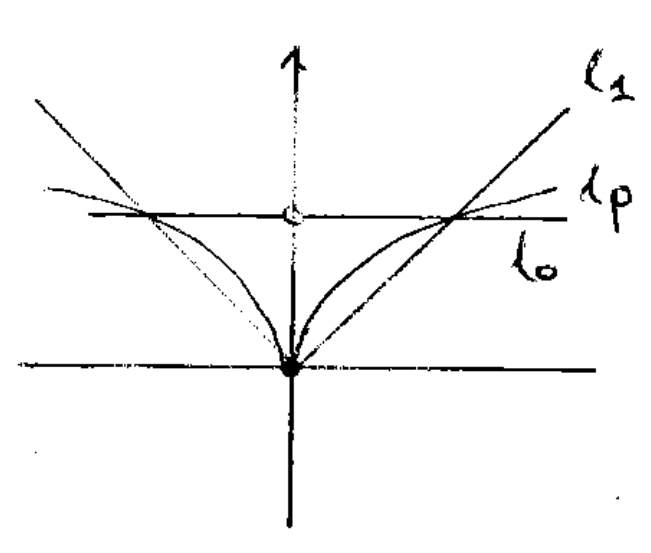
\includegraphics[width=0.32\linewidth]{fig/norms}
    \caption{\small Norms.}
    \label{fig:norms}
\end{figure}

A natural family of functions that interpolate between $l_0$ and $l_1$ is
the $l_p$-quasi-norm,
which is
\begin{equation}
    \|\theta\|_p^p=\sum_{i=1}^d|\theta_i|^p,\quad p\in(0,1).
\end{equation}
This is also known as the bridge penalty in the literature.
It can be verified that
\begin{equation}
    \lim_{\theta\to 0}(|\theta^p|)'=+\infty.
\end{equation}
such a feature is undesirable,
as it implies that $\hat\theta=0$ is always a local minimum to the problem
\begin{equation}
    \min_{\theta\in\real^d}\cL(\theta)+\lambda\|\theta\|_p^p.
\end{equation}
In particular,
there is no hope in bounding the statistical error $\|\hat\theta-\theta^*\|_2$
in general.

\subsection{Theme}

\subsubsection{An Assumption}

To circumvent this difficulty,
we consider regularizers $R_\lambda$ that are separable,
\ie,
\begin{equation}
    R_\lambda(\theta)=\sum_{i=1}^d R_\lambda(\theta_i),
\end{equation}
and satisfy the following properties.
\begin{ass}
Function $R_\lambda:\real\to\real$ satisfies the following:
\begin{enumerate}
    \item $R_\lambda(0)=0$ and $R_\lambda(t)=R_\lambda(-t)$ for all $t\in\real$.
    \item $R_\lambda$ is non-decreasing on $\real_+$.
    \item For $t>0$,
        the function $t\mapsto \frac{R_\lambda(t)}{t}$ is non-increasing in $t$.
    \item $R_\lambda$ is differentiable for all $t\ne0$
        and subdifferentiable at $t=0$ with
        $\lim_{t\searrow0}R_\lambda'(t)=\lambda L$ for some $L>0$.
    \item There exists a $\mu>0$ \st
        $t\mapsto R_{\lambda,\mu}(t)=R_\lambda(t)+\frac{\mu}{2}t^2$ is convex.
\end{enumerate}
\end{ass}

Both (1) and (2) are rather standard.
If $R_\lambda$ is concave on $\real_+$ and satisfies (1),
then it satisfies (3).
Condition (4) rules out those regularizers that have unbounded derivatives
at zero or are not differentiable at some $t\ne0$.
Lastly,
condition (5) sayas that $R_\lambda$ cannot be ``too non-convex''.

An interesting consequence of the above assumption is that
the function $R_\lambda$ is implementing a thresholding rule.
To see this,
define
\begin{equation}
    \lambda^*=\inf_{t>0}\bigg\{\frac{t}{2}+\frac{R_\lambda(t)}{t}\bigg\}.
\end{equation}
Observe that,
\begin{equation}
    0=\argmin_t\bigg\{\frac{(z-t)^2}{2}+R_\lambda(t)\bigg\}\quad
    \text{iff}\quad|z|\le\lambda^*.
\end{equation}
This follows from the fact that
\begin{equation}
    \frac{(z-t)^2}{2}+R_\lambda(t)-\frac{z^2}{2}
        =t\bigg(\frac{t}{2}+\frac{R_\lambda(t)}{t}-z\bigg).
\end{equation}

As a first example,
it can be readily verified that $R_\lambda(t)=\lambda|t|$
satisfies the above properties.
As it turns out,
so does many other widely used regularizers.

\begin{ex}[Smoothly Clipped Absolute Deviation (SCAD)]
\todo
\end{ex}

\begin{ex}[Minimax Concave Penalty (MCP)]
\todo
\end{ex}

\subsubsection{Consequences of Assumption}

Let us now collect some useful consequences of the properties in the assumption.
\begin{pro}
Under the assumption,
$R_\lambda$ is $\lambda L$-Lipschitz.
Moreover,
\begin{equation}
    \lambda L\|\theta\|_1\le R_\lambda(\theta)+\frac{\mu}{2}\|\theta\|_2^2\quad
    \forall\theta\in\real^d.
\end{equation}
\end{pro}
\begin{proof}
\todo
\end{proof}

The next proposition shows how $R_\lambda$ interacts with the $l_1$-norm
on sparse vectors.
\begin{pro}
Under the assumption,
let $\theta\in\real^d$ and $S$ be the index set of the $k$ largest elements
of $\theta$ in magnitude.
Then for any $\xi>0$,
we have
\begin{equation}
    \xi R_\lambda(\theta_S)-R_\lambda(\theta_{S^c})\le
        \lambda L\;\big(\xi\|\theta_S\|_1-\|\theta_{S^c}\|_1\big).
\end{equation}
Moreover,
if $\theta^*\in\real^d$ is $k$-sparse,
then for any $\theta\in\real^d$,
we have
\begin{equation}
    R_\lambda(\theta^*)-R_\lambda(\theta)\le
        \lambda L\;\big(\|\Delta_S\|_1-\|\Delta_{S^c}\|_1\big),
\end{equation}
where $\Delta=\theta-\theta^*$ and $S$ is the index set of the $k$
largest elements of $\Delta$ in magnitude.
\end{pro}
\begin{proof}
\todo
\end{proof}

\subsection{Finale}

Now let us consider the following regularized loss minimization problem.
\begin{equation}\label{eq:h1}
    \min_{\|\theta\|_1\le R}\big\{\cL(\theta)+R_\lambda(\theta)\big\},
\end{equation}
where $R_\lambda$ satisfies the assumption.
Since \eqref{eq:h1} is non-convex in general,
we are interested in bounding the statistical error $\|\tilde\theta-\theta^*\|_2$
for any $\tilde\theta\in\real^d$ satisfying the first-order optimality condition
of \eqref{eq:h1},
which is given by
\begin{equation}
    \big(\nabla\cL(\tilde\theta)+\nabla R_\lambda(\tilde\theta)\big)^T(\theta-\tilde\theta)
        \ge0\quad\forall\|\theta\|_1\le R.
\end{equation}
Toward that end,
we need a \emph{restricted strong convexity} (RSC)-type condition,
as our previous studies suggest.

\subsubsection{RSC Condition}

\begin{define}
We say that $\cL$ satisfies the RSC condition with parameters
$\alpha_1,\alpha_2>0,\tau_1,\tau_2\ge0$, if
\begin{equation}
    \big(\nabla\cL(\theta^*+\Delta)-\nabla\cL(\theta^*)\big)^T\Delta\ge
    \begin{cases}
        \alpha_1\|\Delta\|_2^2-\tau_1\frac{\log d}{n}\|\Delta\|_1^2 &\text{if }~\|\Delta\|_2\le1,\\
        \alpha_2\|\Delta\|_2-\tau_2\sqrt{\frac{\log d}{n}}\|\Delta\|_1 &\text{if }~\|\Delta\|_2\ge1.\\
    \end{cases}
\end{equation}
\end{define}

The RSC condition above consists of two inequalities,
instead of just on in the RSC conditions we introduced before.
It actually subsumes the previously introduced RSC conditions.
Furthermore,
it allows us to tackle more general (non-convex) loss functions.
For further discussions,
see~\cite{loh2015regularized}.

\subsubsection{Statistical Error Bound}

Using the above RSC condition,
we can establish the following result on the statistical error.
\begin{thm}
Suppose that $R_\lambda$ satisfies the assumption,
$\cL$ satisfies the RSC condition with $\alpha_1>\frac{\mu}{2}$,
and $\theta^*$ is feasible for \eqref{eq:h1}.
Provided
\begin{equation}
    \frac{4}{L}\max\bigg\{\|\nabla\cL(\theta^*)\|_\infty,
        \alpha_2\sqrt{\frac{\log d}{n}}\bigg\}\le\lambda\le\frac{\alpha_2}{{6LR}},
\end{equation}
and
\begin{equation}
    n\ge\frac{16R^2\max\{\tau_1^2,\tau_2^2\}}{\alpha_2^2}\log d,
\end{equation}
every $\tilde\theta$ satisfying the first order optimality condition of
\eqref{eq:h1} satisfies
\begin{equation}
    \|\tilde\theta-\theta^*\|_2\le\frac{3\lambda L\sqrt{k}}{2\alpha_1-\mu},
\end{equation}
where $k=\|\theta^*\|_0$.
\end{thm}
\begin{proof}
\todo
\end{proof}


\clearpage
\section{Note I}


\clearpage
\section{Note J}

\subsection{Prelude}

\subsubsection{Recall}

In the past lectures,
we focused on regularized loss minimization problems that have
non-convex loss functions and/or non-convex regularizations.
By stipulating that the loss function satisfies RSC and that
the regularizers is not ``too non-convex'',
we essentially turned the problem into a convex one,
for which standard techniques apply.

\subsubsection{This Lecture}

In this lecture,
we depart from the regularized loss minimization problem and
consider another quite different estimation problem:
the \emph{phase synchronization problem}.
In this problem,
one is interested in recovering a collection of phases $\{e^{i\theta_k}\}$
based on noisy measurements of relative phases $\{e^{i(\theta_j-\theta_k)}\}$.
Specifically,
let
\begin{equation}
    z^*\in T^n\triangleq\{w\in\cpx^n:|w_1|=\cdots=|w_n|=1\}
\end{equation}
be the unknown phase vector we wish to recover.
We have noisy measurements of the form
\begin{equation}\label{eq:probj}
    C_{jl}=z_j^*\bar z_l^*+\Delta_{jl},\quad 1\le j<l\le n,
\end{equation}
where $\Delta_{jk}$ is the noise associated with the $(j,k)$-th measurement.
To recover $z^*$,
it is natural to formulate the following least squares problem,
\begin{equation}
    \hat z \in\argmin_{z\in T^n}\sum_{1\le j<l\le n}|c_{jl}-z_j\bar z_l|^2.
\end{equation}
Using the fact that $|z_j\bar z_l|^2=1$ for any $z\in T^n$,
the above is equivalent to
\begin{equation}\label{eq:j_p}
    \hat z \in\argmax_{z\in T^n}z^HCz,
\end{equation}
where $C_{jj}=1$ for $j=1,\dots,n$.

Note that neither the objective function nor the constraints set of
\eqref{eq:j_p} is convex.
Moreover,
there will be multiple optimal solutions to \eqref{eq:j_p},
because whenever $\hat z$ is optimal,
so is $e^{i\theta}\hat z$ for any $\theta\in[0,2\pi)$.
This also suggests that we can only recover $z^*$ up to a global phase.
Hence,
we define the following distance metric to measure the closeness of
any $z\in T^n$ to the target vector $z^*$,
\begin{equation}
    d_2(z,z^*)=\min_{\theta\in[0,2\pi)}\|z-e^{i\theta}z^*\|_2.
\end{equation}

Following our earlier studies,
a natural first question is to study the estimation performance of $\hat z$
\wrt the metric $d_2$.
As it turns out,
this is rather straightforward.
To begin,
observe from \eqref{eq:probj} that
\begin{equation}
    C=z^*(z^*)^H+\Delta,
\end{equation}
where $\Delta$ is a Hermitian matrix whose diagonal is zero
and its above-diagonal entries are given by $\Delta_{jl}$.
Then,
we have the following,
\begin{pro}\label{pro:j1}
Let $z\in\cpx^n$ be such that $\|z\|_2^2=n$ and $(z^*)^HCz^*\le z^HCz$
(in particular,
these conditions are satisfied by an optimal solution
$\hat z$ to \eqref{eq:j_p}).
Then,
\begin{equation}
    d_2(z,z^*) = \sqrt{2\big(n-|z^Hz^*|\big)}\le\frac{4\|\Delta\|}{\sqrt{n}}.
\end{equation}
\end{pro}
\begin{proof}
By definition,
\begin{equation}
\begin{split}
    d_2(z,z^*)^2=\min_{\theta\in[0,2\pi)\|z-e^{i\theta}z^*\|_2^2}
\end{split}
\end{equation}
\end{proof}

In view of Proposition~\ref{pro:j1},
it is natural to ask if we can find an optimal solution $\hat z$
to \eqref{eq:j_p} efficiently.
Noting that projection onto the non-convex set $T^n$ is efficiently computable,
let us consider the following simple projected gradient scheme,
\begin{equation}
\begin{split}
    w^k &\leftarrow z^k + \frac{\alpha_k}{n}Cz^k, \\
    z^{k+1}&\leftarrow \frac{w^k}{|w^k|},
\end{split}
\end{equation}
where $\alpha_k>0$ is the step size,
and for a vector $w\in\cpx^n$,
\todo


\clearpage
\section{Note K}


\clearpage
\section{Note L}


\medskip

\bibliography{bf}


\end{document}
